\section{Experiments}
This section includes the detailed description of our experiments conducted to analyze the impact of database cracking on query execution performance. We use a similar setup for all performance evaluations. Our main focus is to study the impact of cracking the SELECT operator in memory. In order to identify relative performances, we ran same queries on the same column for all cracker index implementations and compared the results to two baselines: (1) simple scanning which scans the entire column and filters tuples satisfying the query and (2) sorting upfront 

\subsection{Experiment Setup}

\textbf{Hardware:} Amazon AWS server (8 GB memory) and MIT Athena computers (40 GB memory). 

\textbf{Dataset:} An array with one million distinct tuples of range 1 to 10${^6}$. 

\textbf{Workload:} Randomly generated 20000 queries with varying selectivity.

\textbf{Query ranges:} Open (single predicate), closed (lower and upper predicates) and mixed (randomly chosen to be either open or closed).
The predicates are chosen randomly from the range 1 to 10${^6}$.

\textbf{Selectivity:} 0.01 and 0.001. 

\textbf{Minimum Partition Size: } 100 and 1000.The cracker index could potentially become very large for non-repetitive queries and dividing columns further into small pieces would become highly costly. Therefore, we experimented with mentioned minimum partition sizes and not cracking the column any further.
\subsection{Performance of cracking index implementations}

\begin{figure}[h]
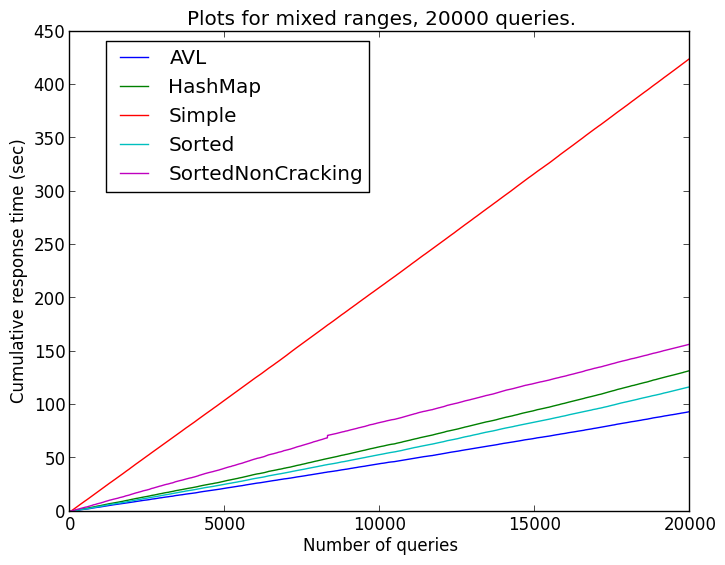
\includegraphics[width=8cm]{figures/mixed20000}
\caption{ADD CAPTION.}
\label{fig:some}
\end{figure}
include graph- -------

\subsubsection{Varying minimum partition size}


This approach simulates a sort based strategy. Upon a first query, the data column we sort the column upon the first query and operates upon the sorted column copy for the queries. This would potentially take O(logN) time for finding the correct start and/or end ranges for the query.

\subsubsection{Varying selectivity}

\textbf{Simple Scanning}
\label{sec:experiments}

